\subsection{Обратная и неявная функция}
\begin{definition}
    Пусть $\lambda\in (0, 1)$, $f: X\rightarrow X$. Тогда $f$ – \textit{сжатие с коэффициентом $\lambda$}, если $\forall x, y\in X$ $\rho(f(x), f(y))\leq \lambda \rho(x, y)$.
\end{definition}

\begin{theorem}
    \textbf{Теорема Банаха о сжатии.}

    Пусть $X$ – полное метрическое пространство, $f: X\rightarrow X$ – сжатие с коэффициентом $\lambda\in (0, 1)$. Тогда существует единственная неподвижная точка (то есть такая точка, что $f(x)=x$).
\end{theorem}

\begin{proof}~
    \begin{enumerate}
        \item \textit{Единственность.}

        Пусть $f(x)=x$ и $f(y)= y$. 
        
        Тогда $\rho(x, y)=\rho(f(x), f(y))\leq \lambda \rho(x, y)\overset{\lambda \in (0, 1)}{\Rightarrow} \rho(x, y)=0\Rightarrow x=y$
        \item \textit{Существование.}

        Возьмем $x_0\in X$ и рассмотрим последовательность $x_{n+1}=f(x_n)$. 
        
        Проверим, что $x_n$ – фундаментальная последовательность, то есть имеет предел, который и будет искомой точкой.

        $\rho(x_n, x_{n+k})=\rho(f(x_{n-1}), f(x_{n+k-1}))\leq \lambda\rho(x_{n-1}, x_{n+k-1})\leq \lambda^2 \rho(x_{n-2}, x_{n+k-2})\leq ... \leq \lambda^n\rho(x_0, x_k)\leq \underset{\rightarrow 0}{\lambda^n}\cdot \underset{=const}{\frac{\rho(x_0, x_1)}{1-\lambda}}$

        $\rho(x_0, x_k)\leq \rho(x_0, x_1) + \underbrace{\rho(x_1, x_2)}_{\leq \lambda\rho(x_0, x_1)} + ... + \underbrace{\rho(x_{k-1}, x_{k})}_{\leq \lambda^{k-1}\rho(x_0, x_1)}\overset{\text{геом. прогр.}}{\leq} \frac{\rho(x_0, x_1)}{1-\lambda}$

        Есть фундаментальность (так как можем сделать $\lambda^n\cdot \frac{\rho(x_0, x_1)}{1-\lambda}<\varepsilon$) $\Rightarrow \exists x_*:= \lim x_n$.

        $f(x_*)=f(\lim x_n)\overset{f\text{ непр.}}{=}\lim f(x_n)=\lim x_{n+1}=x_*\Rightarrow x_*=f(x_*)$
    \end{enumerate}
\end{proof}

\begin{remark}
    Не просто доказали, но еще и предъявили алгоритм – взять произвольную точку и начать итерироваться: применять $f$ к точке, к образу... Тогда с хорошей скоростью будет сходимость к неподвижной точкой.

    Можно, конечно, улучшить скорость, взяв начальную точку получше, но глобально и так будет очень даже неплохо.
\end{remark}

\begin{remark}
    Если $x_*$ – неподвижная точка и $x_n\in X$, то $\rho(x_*, x_n)\leq \lambda^n\frac{\rho(x_0, x_1)}{1-\lambda}$.

    $\underbrace{\rho(x_n, \underbrace{x_{n+k}}_{\rightarrow x_*})}_{\rightarrow \rho(x_n, x_*)}\leq \lambda^n\frac{\rho(x_0, x_1)}{1-\lambda}$ и устремим $k$ к $+\infty$.
\end{remark}

\begin{corollary}
    Пусть $X$ –  полное метрическое пространство, $f, g:X\rightarrow X$ сжатия с коэффициентом $\lambda \in (0, 1)$, $f(x) = x$, $g(y)=y$. Тогда $\rho(x, y)\leq \frac{\rho(f(x), g(x))}{1-\lambda}$.
\end{corollary}

\begin{proof}
    $\rho(x, y)=\rho(f(x), g(y))\leq \rho(f(x), g(x))+\underbrace{\rho(g(x), g(y))}_{\leq \lambda \rho(x, y)}\leq \lambda \rho(x, y)+\rho(f(x), g(x))$
\end{proof}

\begin{definition}
    \textit{Задача Коши для дифференциального уравнения }$\frac{dy}{dx}=f(x, y)$.

    $\left\{\begin{array}{l}
         y'=f(x, y)  \\
         y(x_0)=y_0
    \end{array}\right.$
\end{definition}

Сейчас мы поймем, что если у нас $f$ – достаточно хорошая функция, то задача Коши обязательно имеет единственное решение (правда, только локально, глобально может не быть).

\begin{theorem}
    \textbf{Теорема Пикара.}

    Пусть $f:D\rightarrow \R$ непрерывна, $D\subset \R^2$ открытое, $(x_0, y_0)\in D$ и $|f(x, y)-f(x, \Tilde{y})|\leq M\cdot |y-\Tilde{y}|$ $\forall (x, y)$, $(x, \Tilde{y})\in D$ (то есть при изменении второй координаты функция меняется не сильно). Тогда при некотором $\delta >0$ на отрезке $[x_0 - \delta, x_0 + \delta]$ существует единственная дифференцируемая функция $\varphi$, являющаяся решением задачи Коши $\left\{\begin{array}{l}
         y'=f(x, y)  \\
         y(x_0)=y_0
    \end{array}\right.$.
\end{theorem}

\begin{proof} 
    Предъявим сжатие, для которого $\varphi$ является неподвижной точкой.
    
    $\varphi(x)=y_0 +\int\limits_{x_0}^x f(t, \varphi(t))dt$ – подходит под задачу Коши (дифференцируема функция, значение подходит).

    Возьмем $\overline{\text{B}}_r(x_0, y_0)\subset D$ – компактное множество в $\R^2\Rightarrow$ найдется $K: |f(x, y)|\leq K$ при $(x, y)\in \text{B}_r(x_0, y_0)$. 

    Выберем $\delta > 0$ так, что:
    \begin{enumerate}
        \item $M\delta < 1$.
        \item Если $|x - x_0|\leq \delta$ и $|y -y_0|\leq K\delta$, то $(x, y)\in \text{B}_r(x_0, y_0)$.

        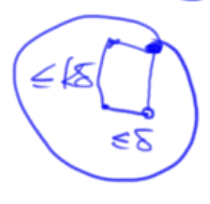
\includegraphics[width=0.1\linewidth]{images/31-05-1.png}
    \end{enumerate}

    Рассмотрим $C_*:=\{\varphi\in C[x_0 - \delta, x_0 + \delta]\mid |\varphi(x) - y_0|\leq K\delta\}\subset C[x_0 - \delta, x_0 + \delta]$. 

    $C_*$ – полное нормированное пространство, $\|\varphi\|=\max\limits_{t\in [x_0 - \delta, x_0 + \delta]} |\varphi(t)|$.

    Определим $T: C_*\rightarrow C_*$: $T(\varphi)= \psi$, где $\psi(x) = y_0+\int\limits_{x_0}^x f(t, \varphi(t))dt$. 
    
    Проверим, что $T$ – это сжатие.

    $|\psi(x)-\Tilde{\psi}(x)|=|\int\limits_{x_0}^x f(t, \varphi(t))dt-\int\limits_{x_0}^x f(t, \Tilde{\varphi}(t))dt|\leq \int\limits_{x_0}^x \underbrace{|f(t, \varphi(t))- f(t, \Tilde{\varphi}(t))|}_{\leq M|\varphi(t)-\Tilde{\varphi}(t)|\leq \|\varphi-\Tilde{\varphi}\|}dt\leq M\delta\|\varphi-\Tilde{\varphi}\|\Rightarrow$ получилось сжатие с коэффициентом $M\delta$<1.

    Тогда по теореме Банаха есть единственная неподвижная точка, которая и является решением задачи Коши.
\end{proof}

\begin{remark}
    Решение задачи Коши существует только локально:

    $\left\{\begin{array}{l}
         y'=-y^2  \\
         y(1)=1
    \end{array}\right.\quad y(x)=\frac{1}{x}$ определено только на $(0, +\infty)$.

    То есть если $D=(-1, 1)\times(-1, 1)$, то на всем отрезке определить не удастся.
\end{remark}

\begin{theorem}
    Пусть $A:\R^n \rightarrow \R^n$ линейный оператор: $\|Ax\|\geq m\|x\|$ $\forall x\in \R^n$, где $m>0$. Тогда $A$ обратим и $\|A^{-1}\|\leq \frac{1}{m}$.
\end{theorem}

\begin{proof}
    Для обратимости нужна инъективность, то есть проверим, что нет точки $\neq 0$, переходящей в $0$.

    Если $Ax=0$, то $\|x\|\leq \frac{1}{m}\|Ax\|=0\Rightarrow x=0\Rightarrow A$ обратимо.

    $\|A^{-1}\|=\sup\limits_{x\neq 0}\frac{\|A^{-1}x\|}{\|x\|}=\sup\limits_{y\neq 0}\frac{\|y\|}{\|Ay\|}\leq \frac{1}{m}$, так как $\frac{\|y\|}{\|Ay\|}\leq \frac{1}{m}$
\end{proof}

\begin{theorem}
    \textbf{Теорема об обратимости оператора, близкого к обратимому.}

    Пусть $A:\R^n\rightarrow \R^n$ обратимый линейный оператор, $\|B-A\|<\frac{1}{\|A^{-1}\|}$. Тогда $B$ обратим, $\|B^{-1}\|\leq \frac{1}{\|A^{-1}\|^{-1}-\|B-A\|}$ и $\|B^{-1}-A^{-1}\|\leq \frac{\|A^{-1}\|^{-1}\|B-A\|}{\|A^{-1}\|^{-1}-\|B-A\|}$
\end{theorem}

\begin{proof}
    $\|Bx\|=\|Ax+(B-A)x\|\geq \|Ax\|-\|(B-A)x\| \geq \frac{\|x\|}{\|A^{-1}\|}-\|B-A\|x\|=\|x\|\underbrace{(\|A^{-1}\|^{-1}\|B-A\|)}_{=m}$ и подставляем $m$ в предыдущую теорему.

    $\|A^{-1}\|\cdot \|Ax\|\geq \|A^{-1}(Ax)\|=\|x\|$

    Последний пункт: $B^{-1}-A^{-1}=B^{-1}(A-B)A^{-1}$ – очевидно, так как норма композиции не превосходит композиции норм. 
\end{proof}

\begin{theorem}
    Пусть $f:\R^n\rightarrow \R^m$ дифференцируема в $\text{B}_r(a)$ и $\|f'(x)\|\leq C$ $\forall x\in \text{B}_r(a)$. Тогда $\|f(x) - f(y)\|\leq C\|x - y\|$.
\end{theorem}

\begin{proof}
    $\varphi(t):=\langle f(x + t(y-x), f(y) - f(x))\rangle$

    Любой отрезок между $x$ и $y$ целиком лежит в круге, то есть при $t\in [0, 1]$ функция определена,

    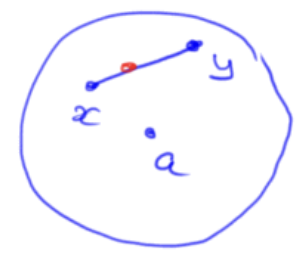
\includegraphics[width=0.15\linewidth]{images/31-05-2.png} 

    $\|f(y)-f(x)\|^2=\varphi(1)-\varphi(0)\overset{\text{th Лагранжа}}{=}\varphi'(\xi)$, $\xi\in (0, 1)$ ($\varphi$ – дифференцируема как композиция, функция от одной переменной)

    $\varphi'(\xi)=\langle f'(x+\xi(y-x))\cdot (y-x), f(y)- f(x)\rangle\leq \|f'(x+\xi(y-x))\cdot (y-x)\| \cdot \| f(y)- f(x)\|\leq \underbrace{\|f'(x+\xi(y-x))\|}_{\leq C}\cdot \|y-x\| \cdot \| f(y)- f(x)\|$
\end{proof}

\begin{theorem}
    \textbf{Теорема об обратной функции.}

    Пусть $D\subset \R^n$ открытое, $f:D\rightarrow \R^n$, $x_0\in D$, $y_0= f(x_0)$, $f$ непрерывно дифференцируема в окрестности точки $x_0$, $A:=f'(x_0)$ обратимо. Тогда существует $U$ и $V$ окрестности точек $x_0$ и $y_0$: $f:U\rightarrow V$ обратима и $f^{-1}:V\rightarrow U$ непрерывно. 
\end{theorem}

\begin{proof} 
    Пусть $G_y(x):=x+A^{-1}(y-f(x))$. 
    
    Выберем $\overline{\text{B}}_r(x_0)$ т.ч. $ \|A^{-1}\|\|A-f'(x)\|\leq \frac{1}{2}$ при $x\in \overline{\text{B}}_r(x_0)$ (так как $\|A^{-1}\|=const$ и $f$ непрерывно дифференцируема, то при $x\rightarrow x_0$ мы можем сделать норму маленькой). 
    
    Тогда $f'(x)$ обратимо при $x\in \overline{\text{B}}_r(x_0)$ (по теореме).

    $G'_y(x)=E+A^{-1}(-f'(x))=E-A^{-1}\cdot f'(x)$

    $\|G'_y(x)\|=\|A^{-1}(A-f'(x))\|\leq \|A^{-1}\|\cdot  \|A-f'(x)\|\leq \frac{1}{2}\Rightarrow\|G'_y(x)\|\leq \frac{1}{2}$ при $\forall x\in \overline{\text{B}}_r(x_0)\Rightarrow \|G'_y(x)-G'_y(\Tilde{x})\|\leq \frac{1}{2}\|x-\Tilde{x}\|$ при $\forall x, \Tilde{x}\in \overline{\text{B}}_r(x_0)\Rightarrow G_y$ – сжатие с коэффициентом $\frac{1}{2}$.

    Хотим понять, что круг перейдет в круг.

    $\|G_y(x)-x_0\|\leq \|G_y(x_0)-x_0\|+\|G_y(x)-G_y(x_0)\|\leq \underbrace{\|A^{-1}(y-f(x_0))\|}_{\leq \|A^{-1}\|\cdot \|y-f(x_0)\|=\|A^{-1}\|\cdot \|y-y_0\|}+\underbrace{\frac{1}{2}\|x-x_0\|}_{\leq \frac{r}{2}\text{ при }x\in \overline{\text{B}}_r(x_0)}$

    Можно выбрать $\text{B}_R(y_0)$, т. ч. $\forall y\in \text{B}_R(y_0)$ $\|A^{-1}\|\cdot \|y-y_0\|< \frac{r}{2}\Rightarrow \|G_y(x)-x_0\|<r$.

    То есть если $y\in\text{B}_R(y_0)$ ($y$ близко к $y_0$), то $G_y(\overline{\text{B}}_r(x_0))\subset  \text{B}_r(x_0)\Rightarrow$ у $G_y$  есть единственная неподвижная точка $x_y\in \text{B}_r(x_0)$:

    $x_y=G_y(x_y)=x_y+A^{-1}(y-f(x_y))\Leftrightarrow A^{-1}(y-f(x))=0\Leftrightarrow f(x_y)=y\Leftrightarrow f(\overline{\text{B}}_r(x_0))\supset \overline{\text{B}}_R(y_0)$

    ($\Leftrightarrow$, так как есть инъективность в силу единственности неподвижной точки)

    Определим окрестности: $V:=\overline{\text{B}}_R(y_0)$, $U:=f^{-1}(V)$, $f:U\rightarrow V$ биекция

    Проверяем непрерывность $f^{-1}$. Пусть $f(x)=y$ и $f(\Tilde{x})=\Tilde{y}$.

    $\|f^{-1}(y)-f^{-1}(\Tilde{y})\|=\|x-\Tilde{x}\|=\|G_y(x)-G_{\Tilde{y}}(\Tilde{x})\|\leq 2 \|G_y(x)-G_{\Tilde{y}}(x)\|=2\|(x+A^{-1}(y-f(x)))-(x+A^{-1}(\Tilde{y}-f(x)))\|=2\|A^{-1}(y-\tilde{y})\|\leq 2\|A^{-1}\|\cdot \|y-\Tilde{y}\|\Rightarrow$ если $y$ близки, то и $x$ близки.
\end{proof}

\begin{theorem}
    \textbf{Теорема о дифференцируемости обратного отображения.}

    Пусть $f:D\rightarrow \R^n$ непрерывно дифференцируемо, $f(x_0)=y_0$, $A:=f'(x_0)$ обратимо, $U$ и $V$  окрестности точек $x_0$ и $y_0$, т. ч. $f:U\rightarrow V$ и $f^{-1}: V\rightarrow U$ непрерывно. Тогда $f^{-1}$ дифференцируемо в точке $y_0$.
\end{theorem}

\begin{proof}
    $f(x_0+h) = f(x_0) + Ah + \alpha(h) \|h\|$, где $ \alpha(h)\rightarrow 0$ при $h\rightarrow 0$.

    $k:= f(x_0+h) - f(x_0)=Ah + \alpha(h) \|h\|$
    
    $\|Ah\|\geq \frac{\|h\|}{\|A^{-1}\|}$, тогда $k\geq \frac{\|h\|}{\|A^{-1}\|} - \|\alpha(h)\| \|h\| \geq \underbrace{(\frac{1}{\|A^{-1}\|} - \|\alpha(h)\|)}_{>0}\cdot \|h\|\Rightarrow$ если $k\rightarrow 0$, то и $h\rightarrow 0$.

    $f^{-1}(y_0+k)-f^{-1}(y_0)=x_0+h-x_0=h=A^{-1}\underbrace{(Ah+\alpha(h) \|h\|)}_{=k}-A^{-1}(\alpha(h) \|h\|)=A^{-1}k-\underbrace{A^{-1}(\alpha(h)) \|h\|}_{=o(\|k\|)}$, так как $\|h\|\leq C\|k\|$
\end{proof}

\begin{corollary}
    В условиях теоремы об обратной функции если $f$ непрерывно дифференцируема, то $f^{-1}$ также непрерывно дифференцируема.
\end{corollary}

\begin{corollary}
    Пусть $f: D\rightarrow \R^n$, $D\subset \R^n$ открытое, $f'(x)$ обратимо $\forall x\in D$. Тогда $\forall G\subset D$ открытого $f(G)$ открыто.
\end{corollary}

\begin{proof}
    Возьмем $y_0\in f(G)\Rightarrow \exists x_0\in G$ т.ч. $f(x_0)=y_0$. Применим теорему об обратной функции: $\exists U$ и $V$ окрестности точек $x_0$ и $y_0$, т.ч. $f:U\rightarrow V$ биекция $\Rightarrow V=f(U)\subset f(G)\Rightarrow y_0$ – внутренняя точка $f(G)\Rightarrow f(G)$ открыта. 
\end{proof}

Пусть $x\in \R^n$, $y\in \R^m$, $(x, y)\in \R^{n+m}$.

\begin{statement}
    Пусть $A: \R^{n+m}\rightarrow \R^n$ линейный оператор, т.ч. $A(h, 0)=0\Rightarrow h=0$. Тогда уравнение $A(x, y)=0$ $\forall y\in \R^m$ имеет единственное решение.
\end{statement}

\begin{proof}
    $h\in \R^n\rightarrow A(j, 0)\in \R^n$ биекция, так как это инъекция (0 переходит только в 0) + размерности совпадают.

    $A(x, y)=0\Leftrightarrow A(x, 0)=-A(0, y)$, так как $(x, y)=(x, 0)+(0, y)$.

    $A(x, 0)$ – биекция $\Rightarrow$ существует единственный $y$.
\end{proof}